\documentclass[a4paper, 12pt]{article}%тип документа

%%%Библиотеки
	%\usepackage[warn]{mathtext}	
	\usepackage[T2A]{fontenc} % кодировка
	\usepackage[utf8]{inputenc} % кодировка исходного текста
	\usepackage[english,russian]{babel} % локализация и переносы
	\usepackage{caption}
	\usepackage{listings}
	\usepackage{multirow}
	\usepackage{amsmath,amsfonts,amssymb,amsthm,mathtools}
	\usepackage{wasysym}
	\usepackage{graphicx}%Вставка картинок правильная
	\usepackage{float}%"Плавающие" картинки
	\usepackage{wrapfig}%Обтекание фигур (таблиц, картинок и прочего)
	\usepackage{fancyhdr} %загрузим пакет
	\usepackage{lscape}
	\usepackage{xcolor}
	\usepackage[normalem]{ulem}
	\usepackage{hyperref}

%%%Конец библиотек




%%%Настройка ссылок
	\hypersetup
	{
		colorlinks=true,
		linkcolor=blue,
		filecolor=magenta,
		urlcolor=blue
	}
%%%Конец настройки ссылок


%%%Настройка колонтитулы
	\pagestyle{fancy}
	\fancyhead{}
	\fancyhead[L]{Лабораторная работа}
	\fancyhead[R]{Талашкевич Даниил, группа Б01-008}
	\fancyfoot[C]{\thepage}
%%%конец настройки колонтитулы

\newcommand{\const}{\mathrm{const}}
\newcommand{\rref}[1]{(\ref{#1})}
\newcommand{\isotope}[2]{$ ^{#2}\mathrm{#1} $}
\newenvironment{comment}{}{}
\newcommand{\picref}[1]{рис. \ref{#1}}
\newcommand{\mbf}{\mathbf}
\newcommand{\gmm}{$\gamma $}
\newcommand{\btt}{$\beta $}
\newcommand{\dlt}{$\delta $}
\newcommand{\Equip}[3]{
	
	\item{\bf #1:} $\Delta = \pm #2\; #3$}
\newcommand{\equip}[1]{
	
	\item{\bf #1}}
\newcommand{\labname}{Исследование энергетического спектра \btt-частиц и определение их максимальной энергии при помощи	магнитного спектрометра} 	% название пиши здесь
\newcommand{\labnum}{5.4.2}		% номер вводи здесь
\renewcommand{\epsilon}{\varepsilon}
\renewcommand{\phi}{\varphi}
\newcommand{\angstrom}{\text{\AA}}

							\begin{document}
						%%%%Начало документа%%%%


%%%Начало титульника
\begin{titlepage}

	\newpage
	\begin{center}
		\normalsize Московский физико-технический институт \\(госудраственный 			университет)
	\end{center}

	\vspace{6em}

	\begin{center}
		\Large Лабораторная работа по квантовой физике\\
	\end{center}

	\vspace{1em}

	\begin{center}
		\large \textbf{Исследование энергетического спектра $\beta$-частиц  [4.2]}
	\end{center}

	\vspace{2em}

	\begin{center}
		\large Талашкевич Даниил Александрович\\
		Группа Б01-008
	\end{center}

	\vspace{\fill}

	\begin{center}
	Долгопрудный \\2022
	\end{center}
	
\end{titlepage}
%%%Конец Титульника



%%%Настройка оглавления и нумерации страниц
	\thispagestyle{empty}
	\newpage
	\tableofcontents
	\newpage
	\setcounter{page}{1}
%%%Настройка оглавления и нумерации страниц


					%%%%%%Начало работы с текстом%%%%%%



	\section{Аннотация}
	\textbf{Цель работы:} исследовать энергетический спектр \btt-частиц при распаде ядер \isotope{Cs}{137} и определить их максимальную энергию.\\
	\textbf{В работе используются:} \btt-источник; Форвакуумный насос; Вакуумметр (фигура номинальная); Магнитная линза со свинцовым фильтром и диафрагмой;Сцинтилляционный счётчик; Источники питания 0,02 А; Компьютер.
	
	\subsection{Теоретические сведения}
	
	\begin{wrapfigure}{}{0.49\textwidth}
		
\includegraphics[width=1.0\linewidth]{Screenshot_1}
		\caption{Форма спектра \btt-частиц при разрешённых переходах}
		\label{fig:screenshot1}
	\end{wrapfigure}
	
	Бета-распадом называется самопроизвольное превращение ядер,	при котором их массовое число нс изменяется, а заряд увеличивается или уменьшается на единицу.В данной работе мы будем иметь дело с электронным \btt-распадом:
	\begin{equation*}
		^A_Z X \leftarrow ^A_{Z+1} X+e^-+\widetilde{\nu},
	\end{equation*}
	при котором кроме электрона испускается антинейтрино. 
	
	Выясним вид энергетического спектра \btt-частиц.
	Во-первых, учтём ЗСЭ:
	\begin{equation}\label{eq:ЗСЭ}
		E_e - E - c k = 0,
	\end{equation}
	где $ c k $ -- энергия нейтрино, $ E_e $ -- максимальная энергия электрона, $ E $ -- кинетическая энергия электрона, а связь между его энергией и импульсом даётся соотношением:
	\begin{equation}\label{eq:E}
		E = c \sqrt{p^2+m^2 c^2} - m c^2.
	\end{equation}
	Условие \eqref{eq:ЗСЭ} можно учесть, введя \dlt-функцию вида
	\begin{equation*}\label{key}
		F = \delta(E_e - E - c k),
	\end{equation*}
	которая по определению не равна нулю только если \eqref{eq:ЗСЭ} выполнено.
	Тогда записать вероятность, что электрон после распада имеет импульс $ d^3 p $, а нейтрино --- $ d^3 k $, можно следующим образом:
	\begin{equation}\label{eq:вероятн}
		d w = D \delta(E_e - E - c k) d^3 p d^3 k = D \delta(E_e - E - c k) p^2 d p k^2 d k d \Omega_e d \Omega_{\widetilde{\nu}},
	\end{equation}
	где $ D $ -- коэффициент пропорциональности, который в этом опыте можно считать константой, $ d \Omega_e $ и $ d \Omega_{\widetilde{\nu}} $ -- элементы телесных углов вылета электрона и нейтрино.
	
	Вероятность искомого события имеет связь со спектром, так как
	\begin{equation}\label{eq:связь_спектра_и_вероятн}
		d N = N_0 d w.
	\end{equation}
	Тогда интегрируем \eqref{eq:вероятн} и учитываем \eqref{eq:связь_спектра_и_вероятн}:
	\begin{equation*}\label{eq:dN}
		d N = \dfrac{16 \pi^2 N_0}{c^2} D p^2 \left(E_e - E\right)^2 d p.
	\end{equation*}
	Дифференцируя \eqref{eq:E}, найдём
	\begin{equation*}\label{key}
		d E = \dfrac{c^2 p}{E+m c^2}d p.
	\end{equation*}
	Тогда окончательно
	\begin{equation}\label{eq:spectre}
		\dfrac{d N}{d E} = N_0 B \sqrt{E\left(E+2 m c^2\right)}\left(E_e-E\right)^2\left(E+m c^2\right), 
	\end{equation}
	что в нерелятивистском приближении упрощается до 
	\begin{equation}\label{eq:simpleSpectre}
		\dfrac{d N}{d E} \approx \sqrt{E} \left(E_e - E\right)^2.
	\end{equation}
	
	Дочерние ядра, возникающие в результате \btt-распада, нередко оказываются возбужденными. Возбужденные ядра отдают свою энергию	либо излучая \gmm-квант, либо передавая избыток энергии одному из электронов с внутренних оболочек атома. Излучаемые в таком	процессе электроны имеют строго определенную энергию и называются конверсионными.
	Соответствующий спектр отображён на рис. \ref{fig:screenshot1}.
		
	\subsection{Экспериментальная установка}
		
	Схема экспериментальной установки отображена на рис. \ref{fig:screenshot2} и \ref{fig:screenshot3}.
	\begin{figure}
		\centering
		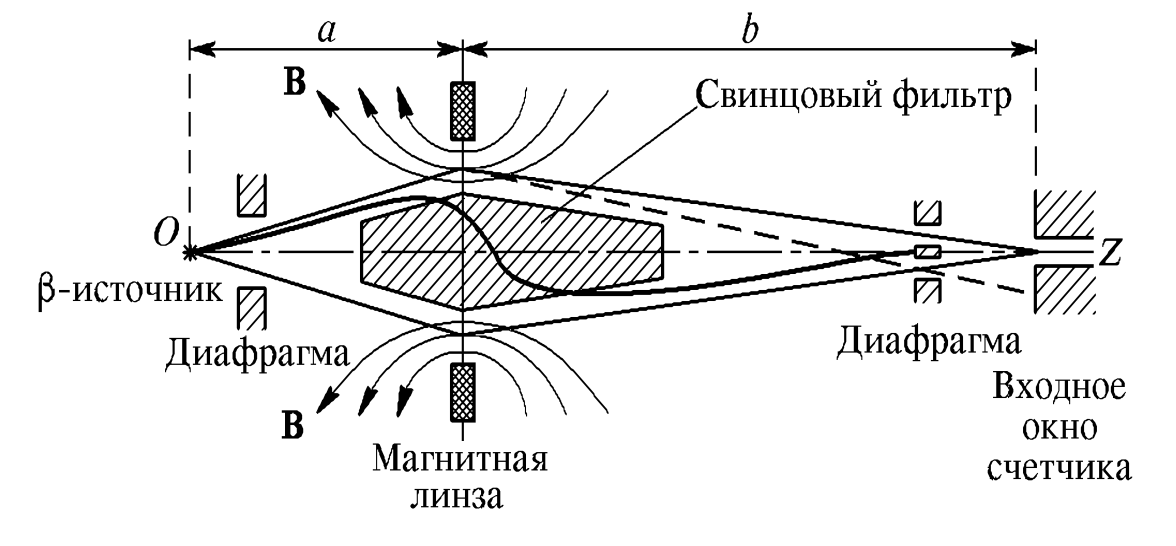
\includegraphics[width=0.7\linewidth]{Screenshot_2}
		\caption{Схема магнитной линзы}
		\label{fig:screenshot2}
	\end{figure}
	\begin{figure}
		\centering
		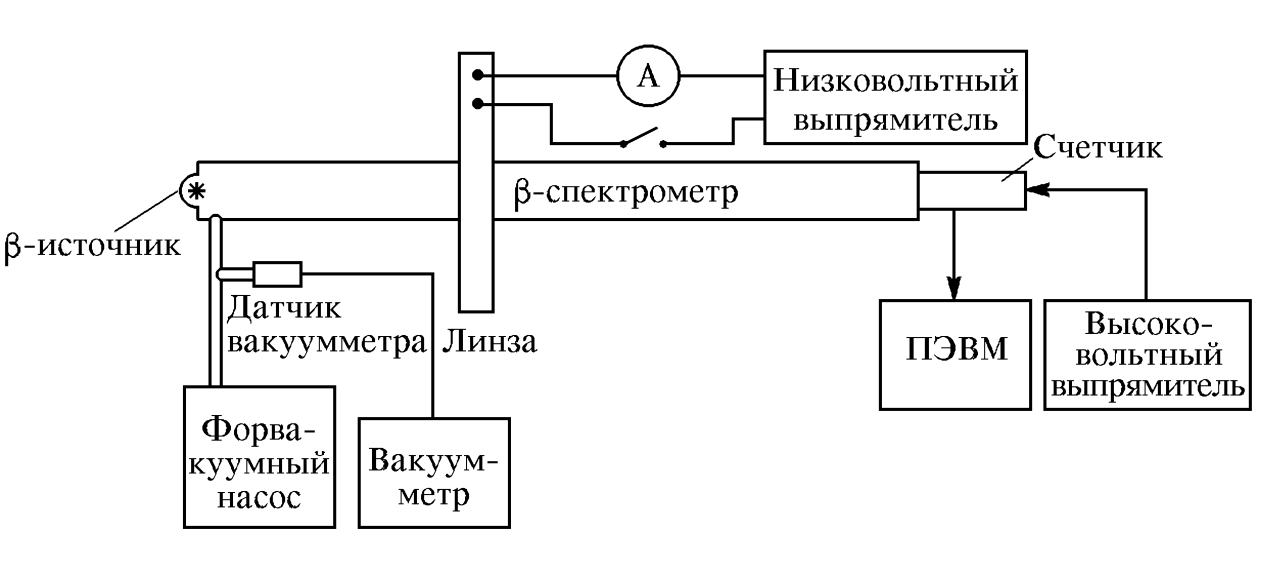
\includegraphics[width=0.7\linewidth]{Screenshot_3}
		\caption{Блок-схема экспериментальной установки}
		\label{fig:screenshot3}
	\end{figure}
	При заданной силе тока на входное окно счетчика фокусируются электроны с определенным импульсом. Электроны, обладающие другими значениями импульса, при этом не сфокусированы и в основном проходят мимо окна. При изменении тока в катушке на счетчик последовательно фокусируются электроны с разными	импульсами, то есть
	\begin{equation*}\label{eq:impulse}
		p_e = k I,
	\end{equation*}
	где $ I $ -- ток катушки.
	Для числа электронов, имеющих импульс $ p_e+\Delta p_e $, можно получить
	\begin{equation*}\label{eq:n_ot_Pe}
		N(p_e) = C W(p_e) p_e,
	\end{equation*}
	где $ C = \const $, $ W(p_e) = d w / d p_e $ находится из формулы \eqref{eq:simpleSpectre}.
	
	\newpage
	\section{Ход работы}
	
	Проведём подробное измерение \btt-спектра, особенно в области конверсионного пика (энергия электронов внутренней конверсии	\isotope{Cs}{137} равна 624 кэВ).	Кроме того, измерим фон.
	
	На месте проведём предварительную обработку результатов эксперимента: учтём фон, прокалибруем спектрометр по конверсионному пику. Кроме того, построим график Ферми-Кюри.
	Полученные данные занесли в таблицу:
	
	\begin{table}[!h]
	\centering
	\begin{tabular}{|c|c|c|c|c|c|}
\hline $\mathrm{I}$, А & $\mathrm{N}$ & $\mathrm{N}-\mathrm{N}_{\text{ф}}$ & $\mathrm{p}$, кэВ/c & $\mathrm{T}$, кэВ & mkFermi \\
\hline 0 & $1.419$ & $1.3072$ & 0 & 0 & 0 \\
\hline $0.2$ & $1.216$ & $1.1041$ & $62.8$ & $3.8$ & 0 \\
\hline $0.4$ & $1.199$ & $1.0874$ & $125.5$ & $15.2$ & 0 \\
\hline $0.6$ & $1.549$ & $1.4372$ & $188.3$ & $33.6$ & $208.8066$ \\
\hline $0.8$ & $2.282$ & $2.1702$ & $251.1$ & $58.3$ & $254.3698$ \\
\hline 1 & $5.481$ & $5.3687$ & $313.8$ & $88.7$ & $369.5900$ \\
\hline $1.2$ & $9.862$ & $9.7499$ & $376.6$ & $123.8$ & $401.3325$ \\
\hline $1.4$ & $11.994$ & $11.8820$ & $439.4$ & $162.9$ & $355.7609$ \\
\hline $1.6$ & $14.476$ & $14.3641$ & $502.1$ & $205.4$ & $323.0977$ \\
\hline $1.8$ & $14.876$ & $14.7639$ & $564.9$ & $250.7$ & $274.8373$ \\
\hline 2 & $15.659$ & $15.5471$ & $627.7$ & $298.4$ & $241.3139$ \\
\hline $2.2$ & $14.476$ & $14.3641$ & $690.5$ & $348.0$ & $200.3917$ \\
\hline $2.4$ & $12.161$ & $12.0486$ & $753.2$ & $399.2$ & $159.7265$ \\
\hline $2.6$ & $8.079$ & $7.9673$ & $816.0$ & $451.8$ & $112.0472$ \\
\hline $2.8$ & $4.698$ & $4.5857$ & $878.8$ & $505.5$ & $71.1942$ \\
\hline 3 & $3.915$ & $3.8028$ & $941.5$ & $560.3$ & $56.4181$ \\
\hline $3.05$ & $8.446$ & $8.3338$ & $957.2$ & $574.1$ & $90.5265$ \\
\hline $3.1$ & $13.86$ & $13.7477$ & $972.9$ & $587.9$ & $116.9774$ \\
\hline $3.15$ & $19.723$ & $19.6115$ & $988.6$ & $601.9$ & $138.2433$ \\
\hline $3.2$ & $24.388$ & $24.2758$ & $1004.3$ & $615.8$ & $151.1093$ \\
\hline $3.3$ & $23.538$ & $23.4262$ & $1035.7$ & $643.9$ & $141.6182$ \\
\hline $3.35$ & $19.09$ & $18.9785$ & $1051.4$ & $658.0$ & $123.8706$ \\
\hline $3.4$ & $14.676$ & $14.5640$ & $1067.1$ & $672.1$ & $105.0884$ \\
\hline $3.45$ & $9.345$ & $9.2333$ & $1082.8$. & $686.3$ & $79.8182$ \\
\hline $3.6$ & $2.399$ & $2.2868$ & $1129.8$ & $729.0$ & $28.1231$ \\
\hline $3.8$ & $0.983$ & $0.8708$ & $1192.6$ & $786.5$ & $0.0$ \\
\hline
\end{tabular}
	\caption{Все данные}
	\label{tab:raw}
\end{table}

\newpage

	$N_{\text{ф}}$, полученное при обработки данных на компьютере:
	\[N_{\text{ф}} = 1.2581,\ dN_{\text{ф}} = 0.112\]
	
	Построим два графика: $ N = F(I) $ на рис. \ref{fig:graph1} и $ \sqrt{N - N_\text{ф}}/p^{\frac{3}{2}}\left[\text{мкФерми}\right] = F(T) $.
	
	\begin{figure}[!h]
		\centering
		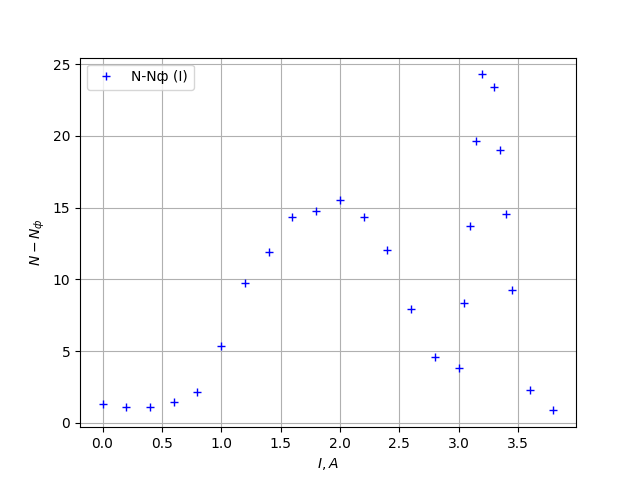
\includegraphics[width=0.9\linewidth]{1.png}
		\caption{График зависимости числа частиц от тока $J$}
		\label{fig:graph1}
	\end{figure}
	
	\begin{figure}[!h]
		\centering
		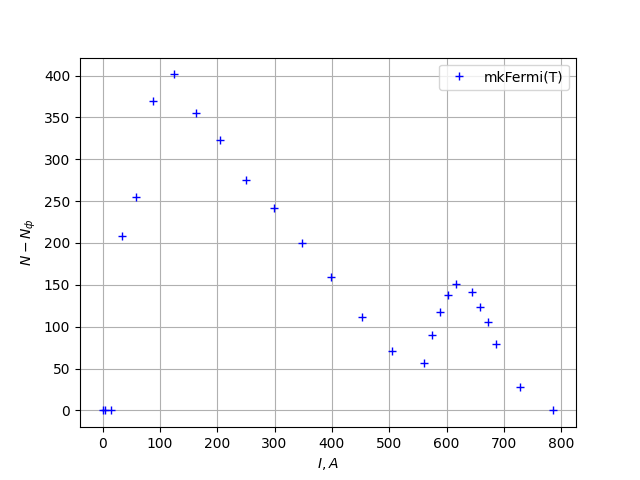
\includegraphics[width=0.9\linewidth]{2.png}
		\caption{График Ферми-Кюри}
		\label{fig:graph2}
	\end{figure}
	
	Проанализировав график получим, что пик при $ I = 3.25\; \text{А} $.
	
	По второму графику, принимая во внимание только точки в средней части и экстраполируя полученную прямую до оси абсцисс, найдём граничную энергию \btt-спектра:
	\[E_\beta^\mathrm{max} = - \dfrac{a}{b} = 612\pm 4 \; \text{кэВ}.\]

	Стоит принять во внимание, что в экстраполяции принимала участие только центральная часть графика, так как данные начальной части имеют существенные погрешности и вообще не очень точны, так как малы энергии электронов, и начинает действовать сила Кулона. Конечная часть графика не выходит на прямую после конверсионного пика, так как блоки питания не могли дать достаточный ток, и крайние точки снять не удалось.
	
	\subsection{Оценка погрешностей}
		
		\label{sec:error}
		
	Точная оценка для величины $ N $, даже из статистических соображений, невозможна, так как во-первых, для каждого опыта сделано только одно измерение, а во-вторых, неизвестна инструментальная погрешность сцинтиллятора и установки в целом. Поэтому считаем погрешность величины $ N $ равной погрешности $ N_{\text{ф}} $, так как только её можно выяснить достаточно достоверно.
		
		\begin{equation*}\label{key}
			\sigma_{N_{\text{ф}}} = 0,04 \;\text{c}^{-1}.
		\end{equation*}
		
	Оценка косвенных погрешностей проводится при помощи пакета \emph{Wolfram Mathematica} по общей формуле:
	\begin{equation}\label{eq:погрешности}
		\Delta_{u(x, y, z, \ldots)}^2 = f'^2_{x} \Delta_x^2 + f'^2_y \Delta_y^2 + f'^2_z \Delta_z^2 + \ldots,
	\end{equation}
	
	Статистическая погрешность для среднего значения $ N_\text{ф} $ может быть вычислена по формуле стандартной ошибки среднего
	\begin{equation}\label{eq:stat}
		\sigma_{N_{\text{ф}}} = \sqrt{\dfrac{1}{n (n-1)} \sum_{i=1}^{n}\left( (N_{\text{ф}})_i - N_{\text{ф}} \right)^2 }.
	\end{equation}
	
	\section{Вывод}
	
	По результатам работы изучили энергетический спектр \btt-частиц и нашли значение максимальной энергии для электрона при \btt-распаде :
	
	\[E_\beta^\mathrm{max} = 612\pm 4 \; \text{кэВ}.\]


	\begin{thebibliography}{3}
		\bibitem{Siv} Сивухин Д. В. \emph{Общий курс физики. Том 5}, 1989
		\bibitem{chp} Фаддеев М. А., Чупрунов Е. В. \emph{Лекции по атомной физике}, 2008
		\bibitem{tsip} Ципенюк Ю. М. \emph{Квантовая микро- и макрофизика}, 2006
		\bibitem{max} Игошин Ф. Ф., Самарский Ю. А., Ципенюк Ю. М. \emph{ЛАБОРАТОРНЫЙ ПРАКТИКУМ ПО ОБЩЕЙ ФИЗИКЕ. Квантовая физика: Учеб, пособие для вузов}; Под ред. Ципенюка Ю.М.
	\end{thebibliography}


\end{document}
